\documentclass{article}
\usepackage[margin=2cm]{geometry}
\usepackage{float}
\usepackage{graphicx}

% Paragraph settings
\setlength{\parskip}{10pt plus 1pt minus 1pt
\setlength{\parindent}{0cm}}

\begin{document}
\title{CS26410 - Assignment 3 \\ Robotic Hide and Seek}
\author{Samuel Jackson \\ \texttt{slj11@aber.ac.uk}}
\date{\today}
\maketitle

\section{Introduction}
Assignment three for CS26410 required us to develop a collection of robotic controllers for use with the Pioneer robots in the ISL which could be used to play a game of hide and seek. This document details the solution that I have provided along with a discussion of its performance using trial runs on real robots.

\section{Discussion of the Algorithms Used}
In the development of this assignment I have used several different techniques and algorithms to solve the problems outlined in the assignment brief. For each of the major problems to be solved in the brief I have supplied a description of my approach to finding a solution.

\subsection{Mapping Techniques}
The first and most important component of the solution was to be able to create a map of the robots environment. The easiest approach to create a simple map of the environment was to create an occupancy gird of the world split into 60x60cm cells in which the robot could fit. As the robot moves through the world, it checks the readings from its sonar array and updates the likelihood that a cell is a wall using the range measured from the sensors. When the robot receives a reading that falls outside the area of the existing grid, my program will dynamically resize the grid to add more cells in the direction of the new reading.

In the previous assignment this mapping was done using a purely random walk. While this approach worked well, it had the major drawback of not having a way to finish mapping unless a human actively told it to stop. In this assignment I decided to take a more structured approach to mapping the environment by utilising depth first and A* search techniques.

Using the new mapping algorithm the robot moves 60cm at a time from one cell to the next while still reading input for its sensors and updating the occupancy grid. When the robot moves into a new cell it checks each of its neighbours to see if they have been discovered or visited. If neither of these conditions are true the robot will add the cell to its "frontier" to come back and look at later. The robot then attempts to keep moving forwards unless there is an obstacle in the way. If there is an obstacle in the way then it will attempt to move into cells on the left or right of it. If the robot hits a dead end it will take the next cell off the frontier and perform an A* search to find the quickest path from the current cell back to the next unexplored cell. The mapping algorithm with continue in this way until there are no more unexplored cells and hence the map is complete.

This technique proved to be fairly suitable to the problem as it ensured that, presuming the world is closed, the robot would eventually map all of it. To ensure that the same parts of the map would not be remapped I turned off the map updating function when the robot was backtracking. While I realise that the use of the A* function is not strictly necessary as backtracking could be implemented with a simple depth-first search, it speeds up map creation considerably by not having to move back through every single previous cell, but instead taking the shortest route to the next unvisited cell.

\subsection{Localization}
After a map of the environment has been created it can be used to aid the robot when hiding or seeking. Note that my map making application saves the generated map as a CSV file which can be loaded into the hiding and seeking programs for reference later.

When I start the hider application, it loads the saved map from file and converts it a map consisting of 0,1 or -1; where 0 is a floor, 1 is a wall and -1 is "undefined" space which we can ignore. To the raw map (containing the original floating point values) to a more structured map I use a threshold value to ensure that cells which might have been incorrectly marks as being slightly occupied are not treated as walls. In this project I am using Otsu's method of thresholding to find the point that minimizes intra-class variance between what can be labelled as a wall and a floor.

In order to localize our self in this map we can begin mapping our environment to build up a picture of what is currently around the robot. I can then use this information and compare each cell in the new map with the existing map to see if it uniquely matches up. If the there is a single unique match then we have localized the robot inside the map. If there are no matches or multiple matches, the program will continue mapping until the grid expands and then attempt to localize again, or until the entire world has been mapped (if we've mapped the whole world again then we clearly must be localized in the environment).

This method works on the basis that at some point in the map there will emerge a definitive landmark that can only match as single arrangement of cells in the pre-existing map. However, there are several problems with the approach that make it less suitable when deployed in the real world. One is the fact that the time complexity of comparing the whole pre-existing map to the newly generated map information multiple times is hardly efficient. Secondly, this approach will not work if the robot is not placed such that the newly generated grid matches up with the existing map. For example, imagine a corridor three cells wide. The robot could be put in such a position that it thinks the corridor is only two cells wide. This localization method would fail in this scenario because of this section of the map would never sync up with the existing map.

\subsection{Finding a Hiding Spot}
Once a reference map has been generated and the robot can localize within it, the robot can now find a good spot to "hide". In my solution, a hiding spot is found by evaluating all floor cells on the grid and checking how far each of the neighbouring walls is. The further away the wall is the more visible the square is and the higher its score. After evaluating all potential positions the program simply picks the cell with the lowest score and uses A* to find the shortest path from the current position to the hiding spot.

This solution seems like a fairly suitable considering the technology available on the Pioneers. There is only very limited information that can be gleaned the Pioneer robots with which to base a solution on and this method is always guaranteed to return a decent solution regardless of the size or shape of the environment providing the map and localization is correct.

\subsection{Finding Map Differences}
The final major problem to be solved was finding a hidden robot within a new map when compared with a reference map. To solve this problem my robot will simply remap the environment and load the reference map, apply the respective thresholds and then compare each point in each map to check if it had changed. The program then outputs a list of points that differ between the two maps.

\section{Trail Runs}

\subsection{Making a Map}

This section documents a number of trials runs of my application carried out on the Pioneer robots in the ISL. For the first trail run, I ran the map maker program to get the Pioneer robot to generate a map of the environment. This run was carried out in a small environment and is shown in the following image.

\begin{figure}[H]
\centering
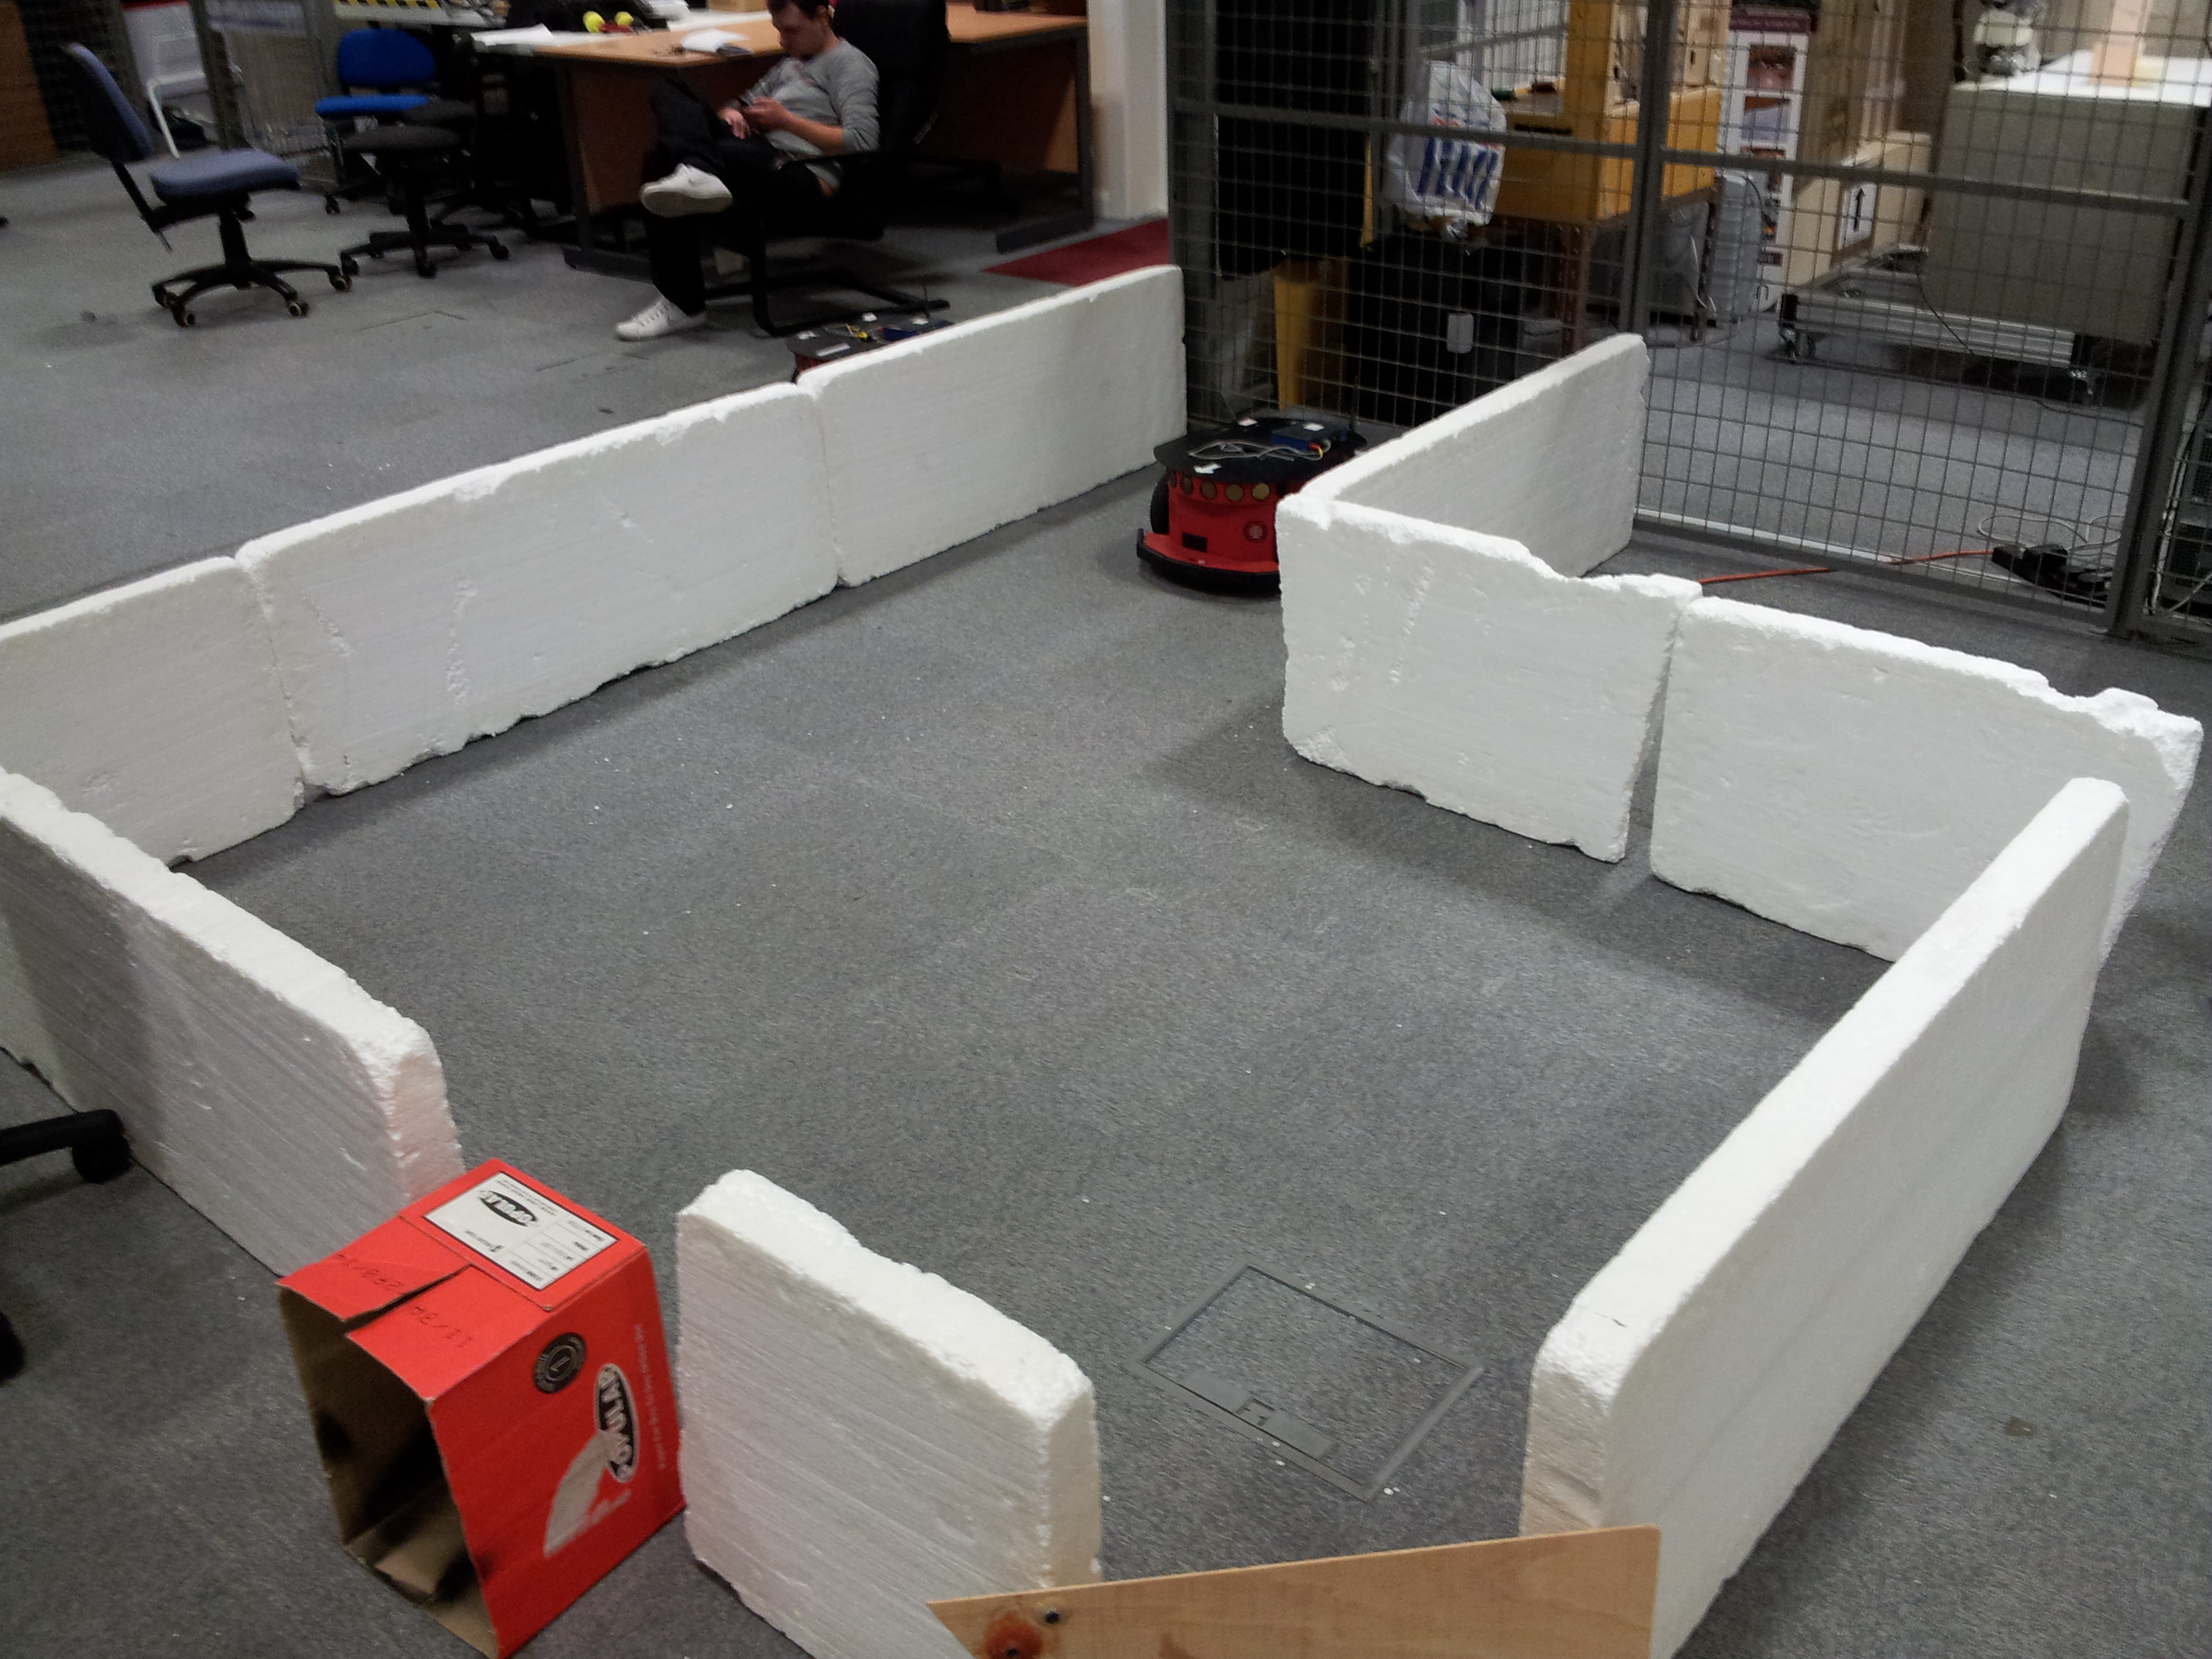
\includegraphics[width=0.5\textwidth]{img/robot_pics/20130416_132221.jpg}
\caption{Pioneer robot at start point in a simple environment.}
\label{fig:robot-map-start}
\end{figure}

The robot then proceeded to map the environment by moving approximately 60cm at a time. The underlying movement system does not require the robot to move exactly 60cm forwards and if it does not move exactly this distance then it will add the difference onto the next movement to help correct for errors over time.

\begin{figure}[H]
\centering
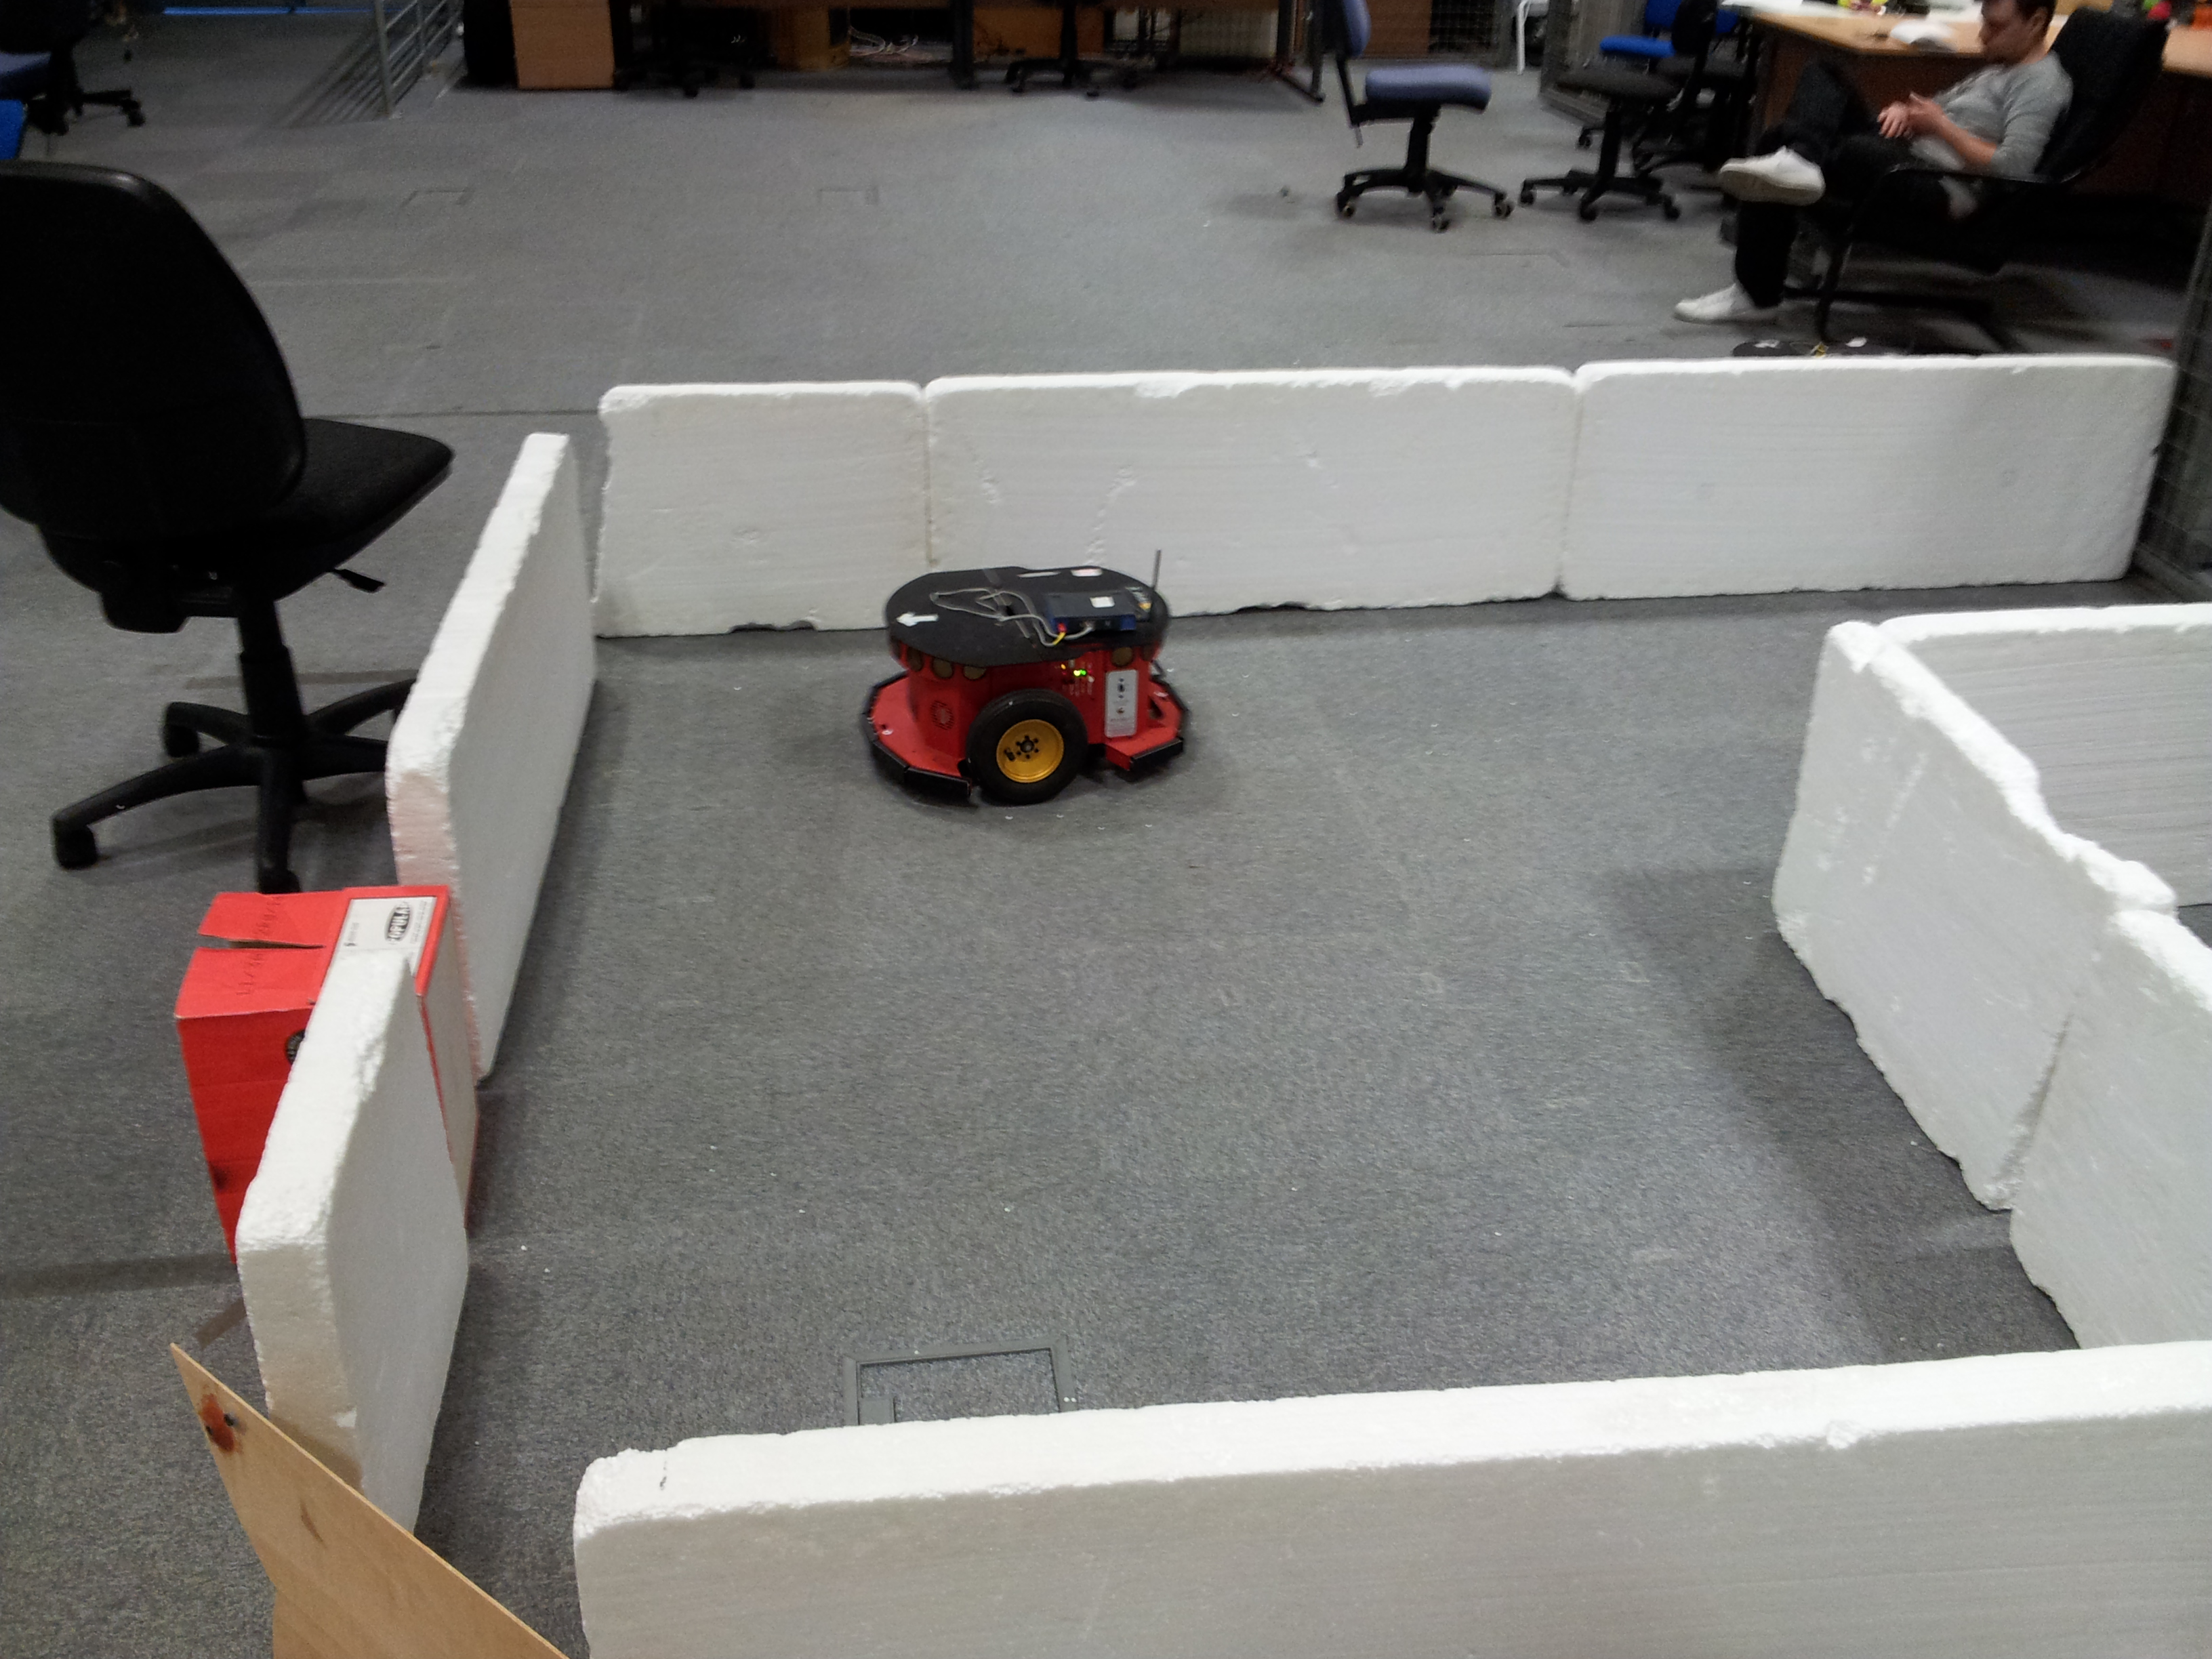
\includegraphics[width=0.5\textwidth]{img/robot_pics/20130416_132253.jpg}
\caption{Pioneer robot after moving forward in the environment.}
\label{fig:robot-map-moved}
\end{figure}

Likewise, when the robot turns it only attempts to turn within 5 degrees either side of the target angle but will correct any error by adding it onto the next turn it performs. An example of an inaccurate turn is shown in figure \ref{fig:robot-map-turned}.

\begin{figure}[H]
\centering
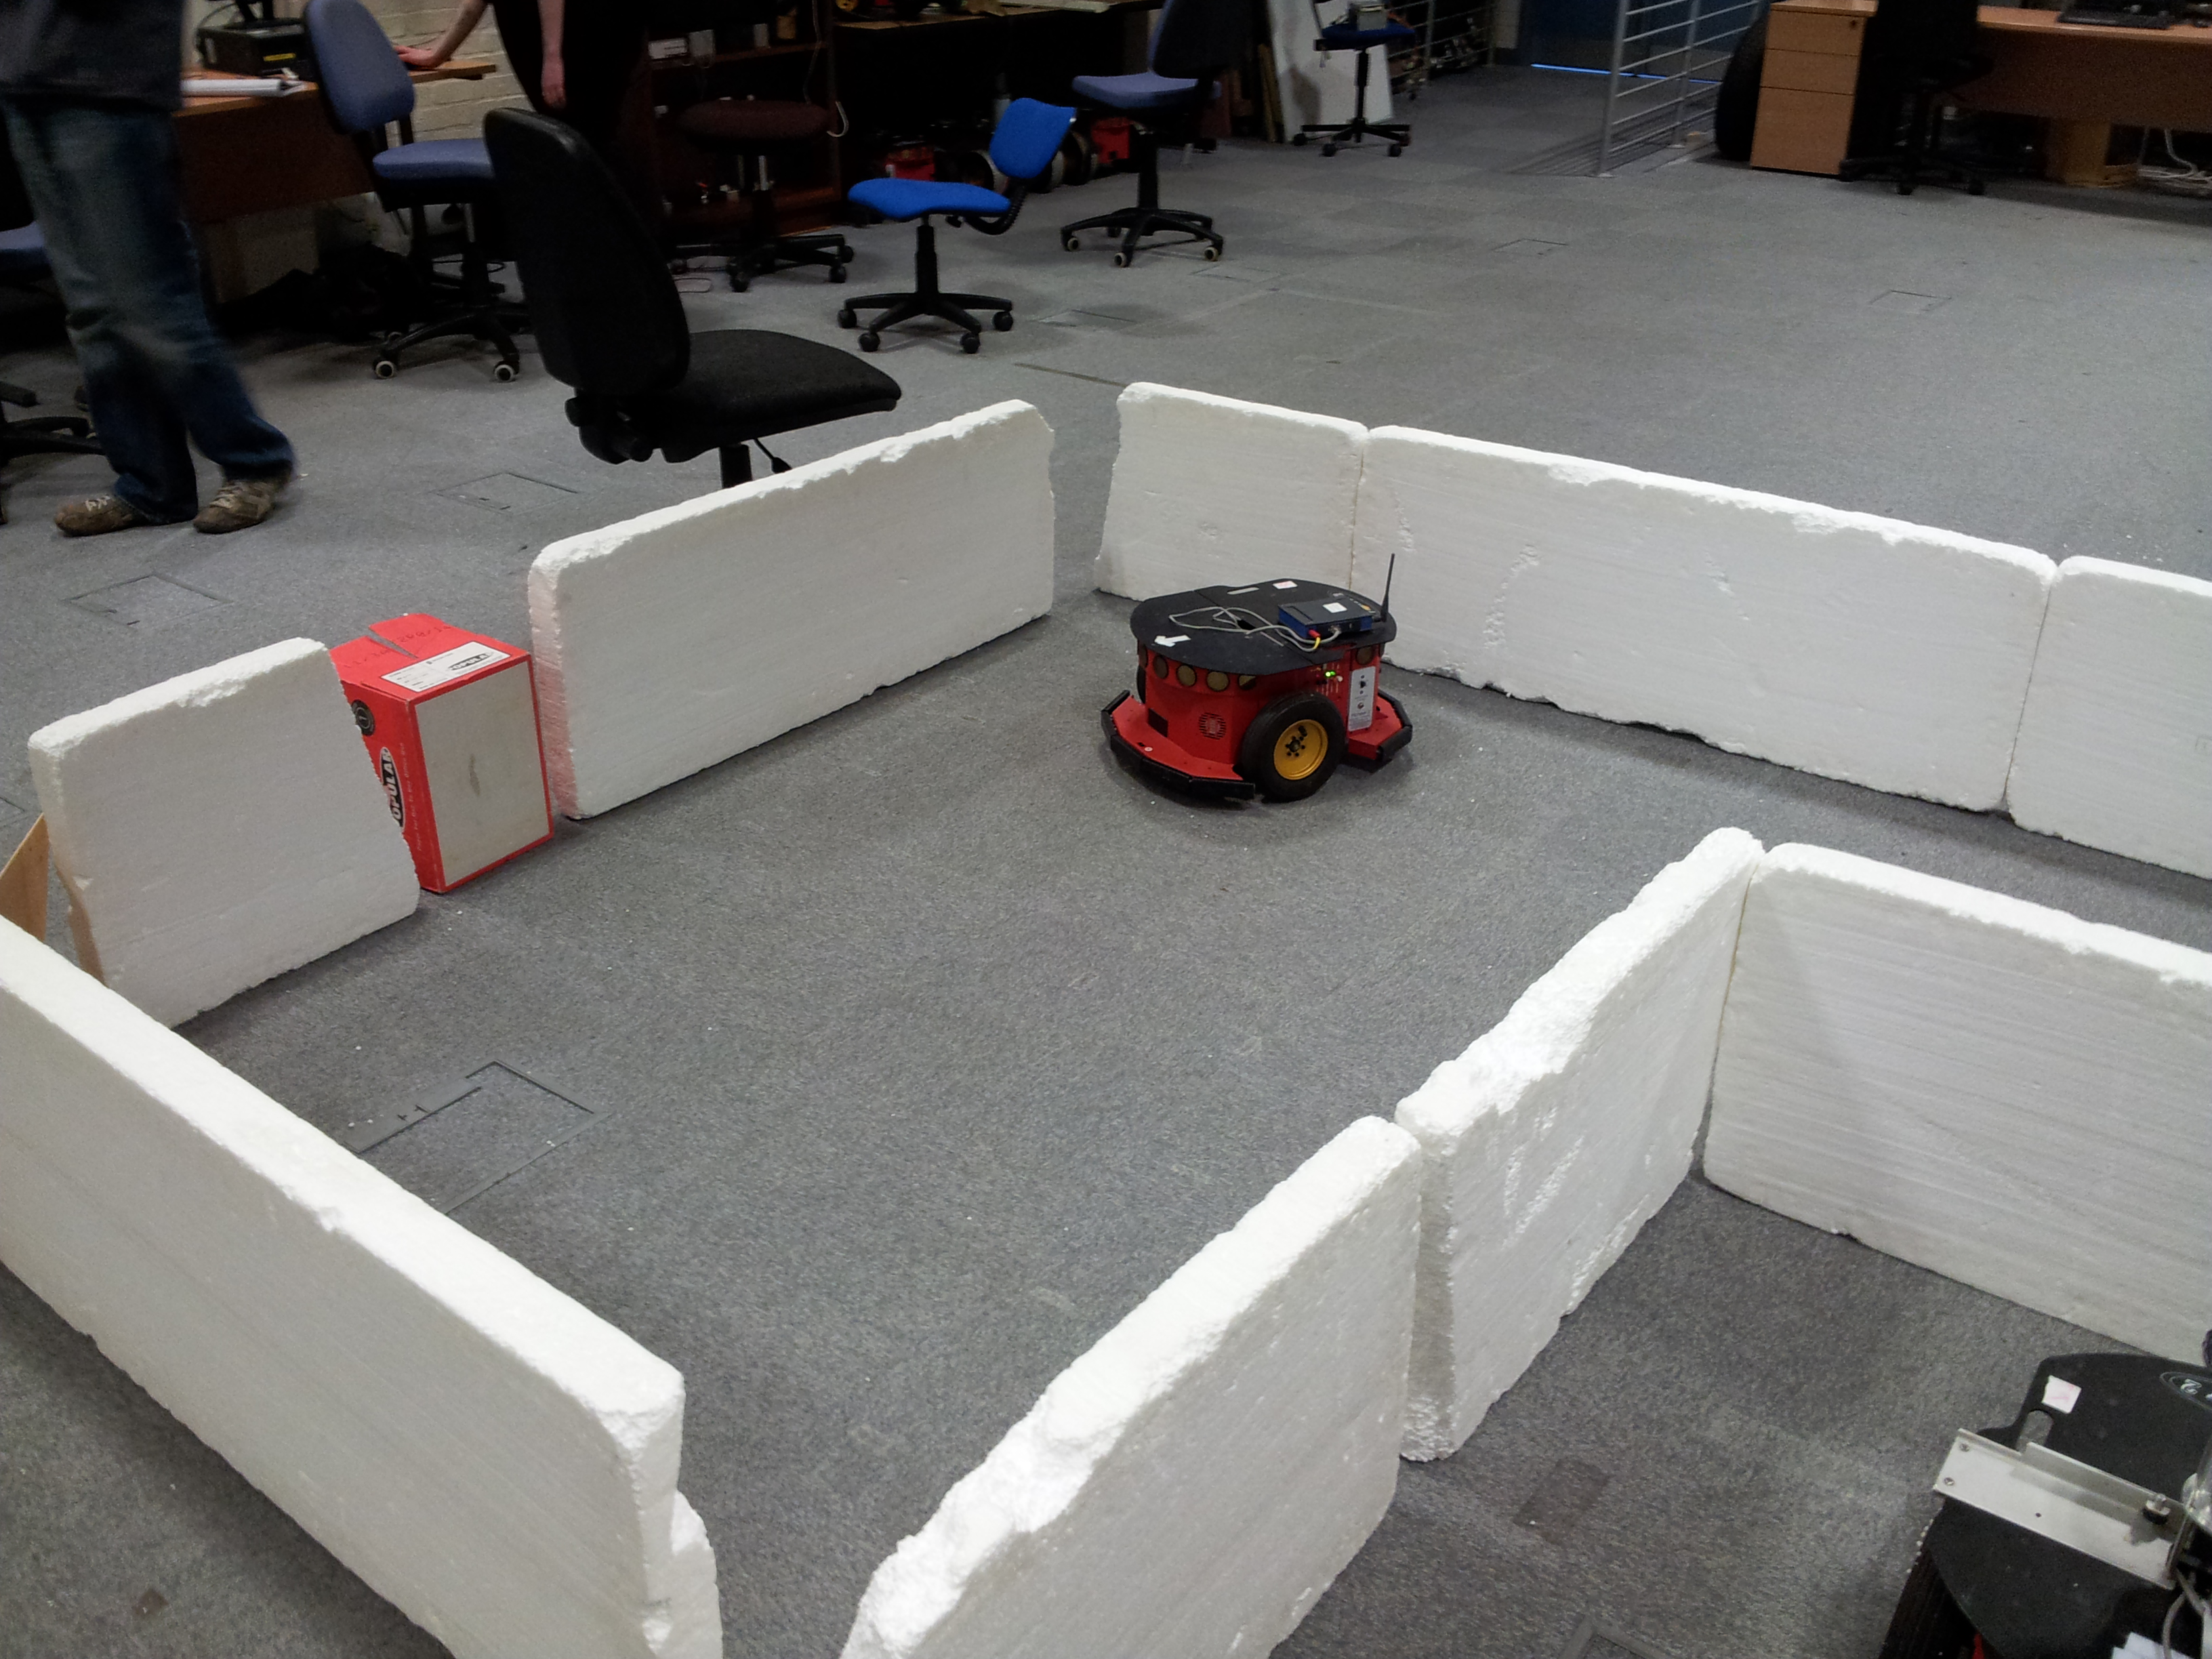
\includegraphics[width=0.5\textwidth]{img/robot_pics/20130416_132300.jpg}
\caption{Pioneer robot after performing a turn. This angle was meant to be approximately 90 degrees but with up to 5 degrees of error.}
\label{fig:robot-map-turned}
\end{figure}

The robot will continue to map until it runs out of squares that have not yet been visited. Below is an image of the robot after it has finished mapping and a screen shot of map produced by the robot. Compare the screen shot in figure \ref{fig:robot-map-run1} with the image of the initial set-up in figure \ref{fig:robot-map-start}.

\begin{figure}[H]
\centering
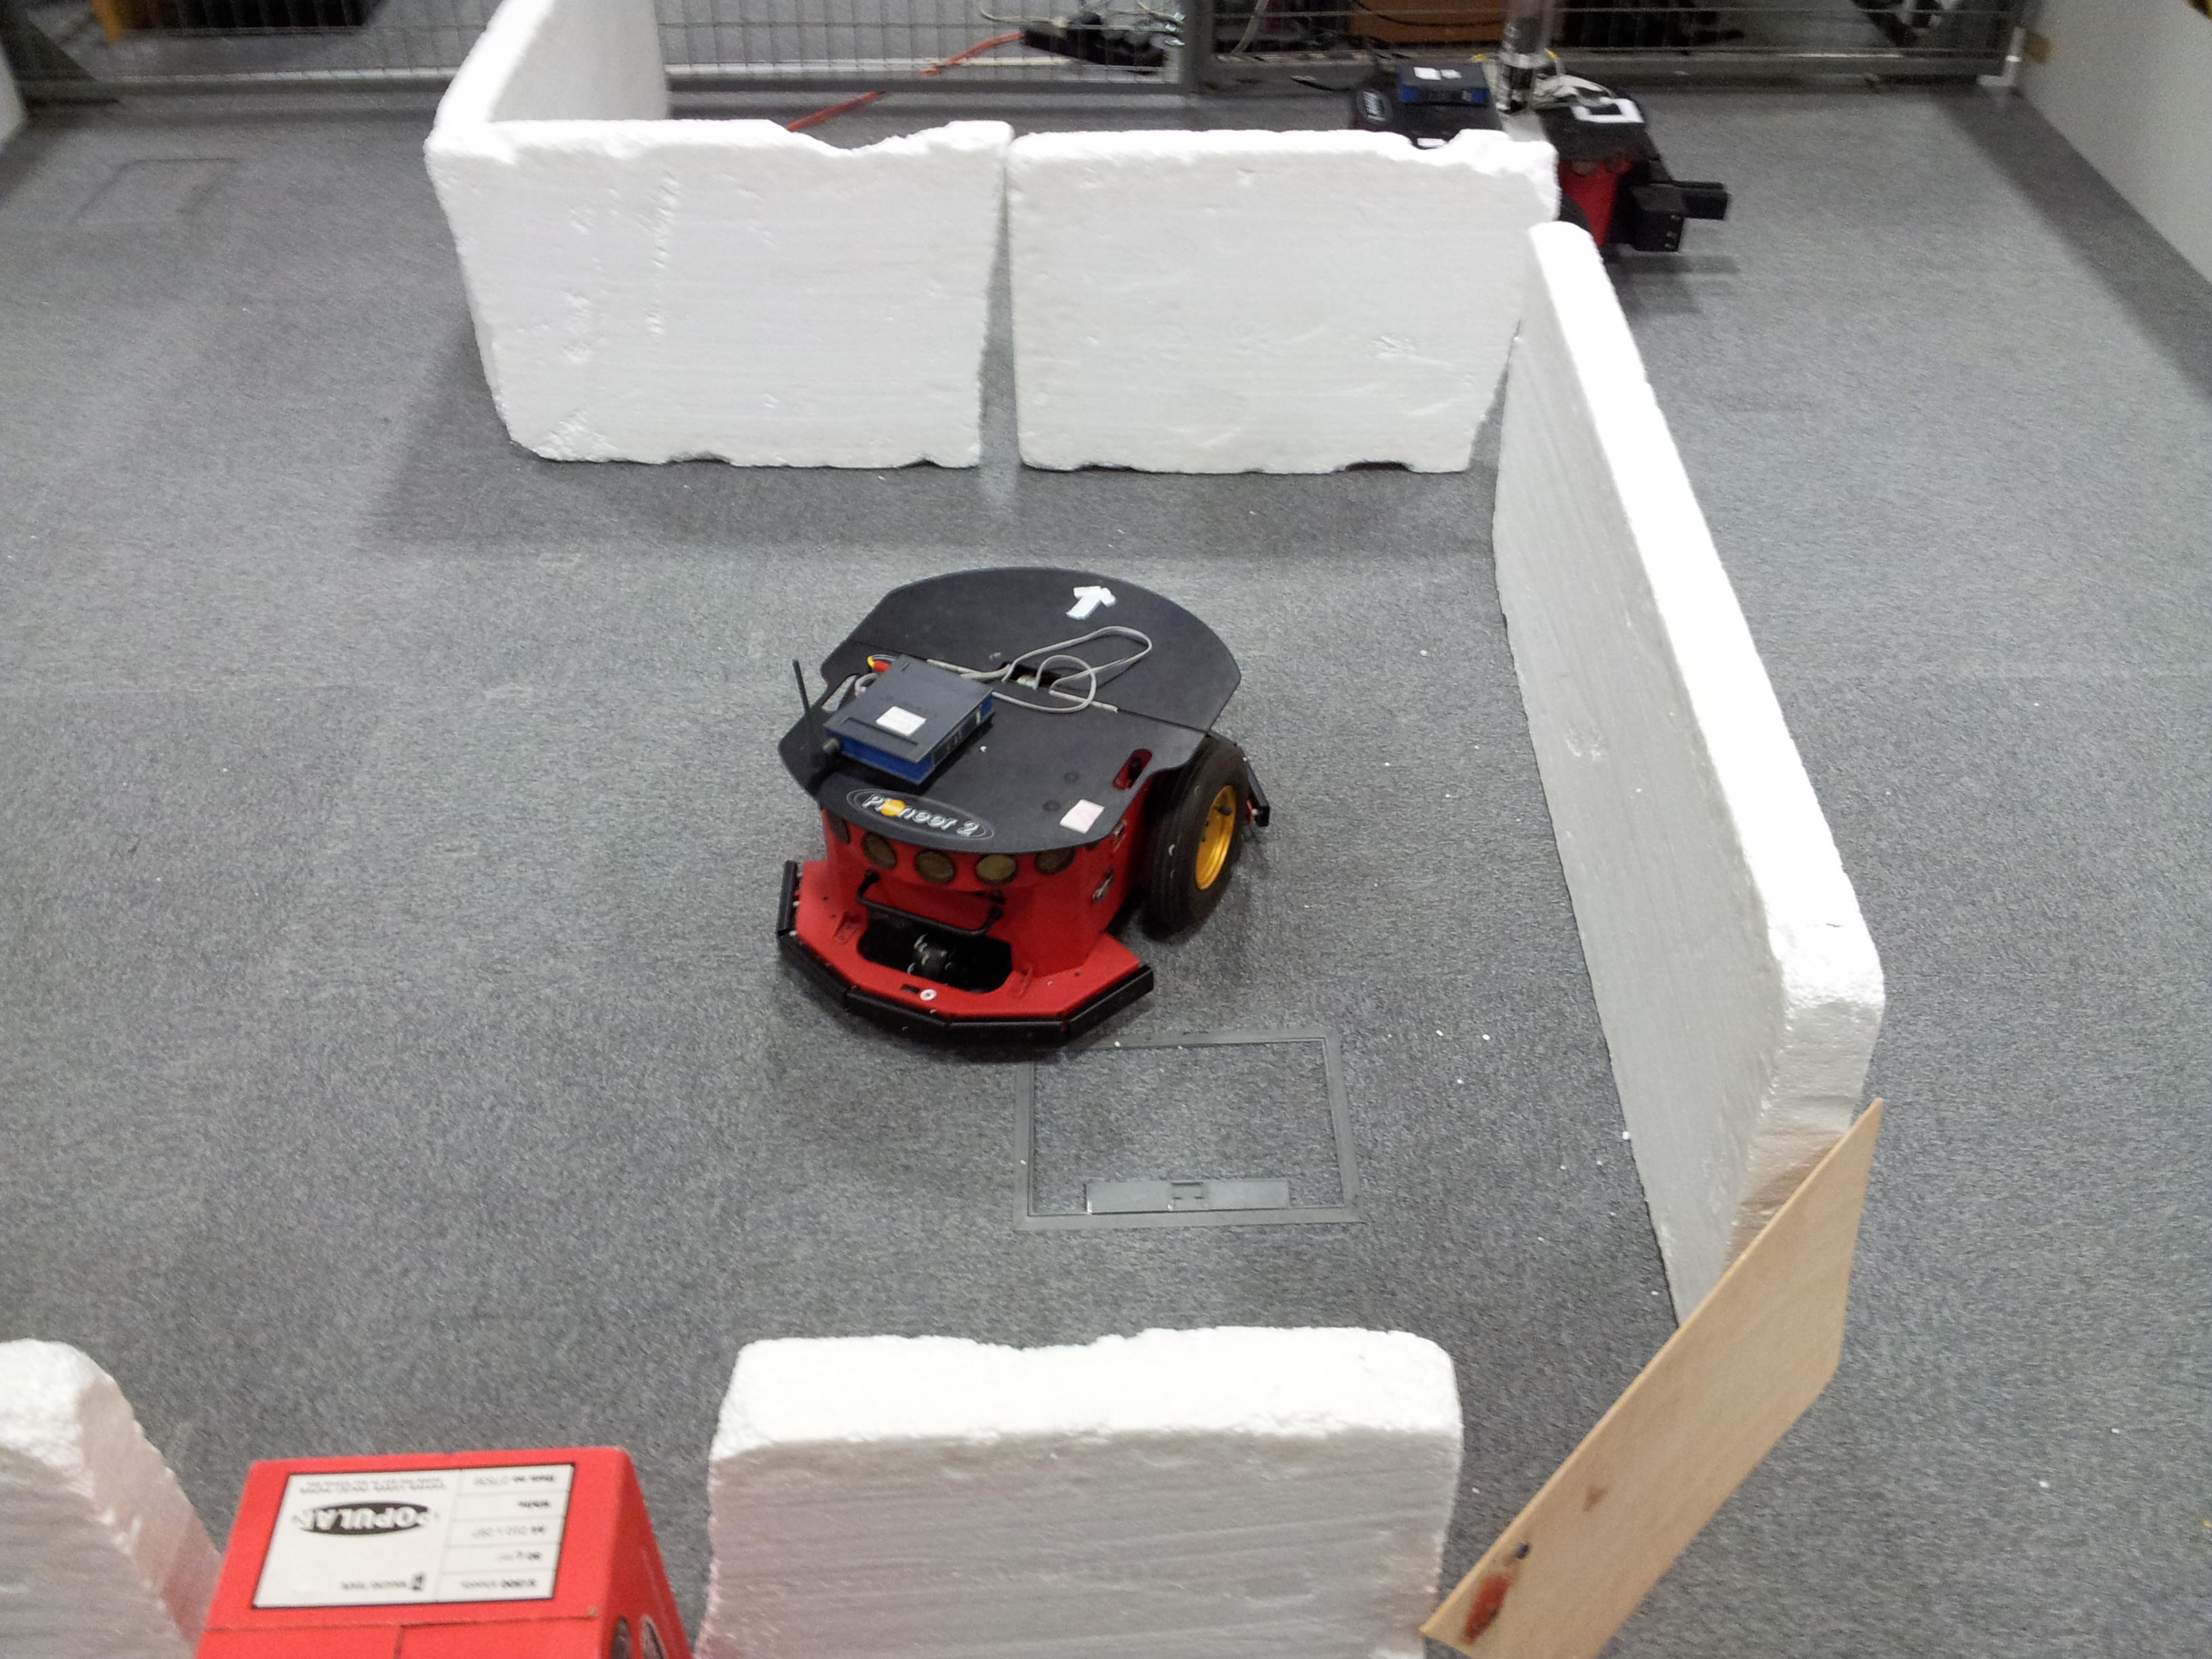
\includegraphics[width=0.5\textwidth]{img/robot_pics/20130416_133043.jpg}
\caption{Pioneer robot after it has visited every part of the environment and finished mapping.}
\label{fig:robot-map-finished}
\end{figure}

\begin{figure}[H]
\centering
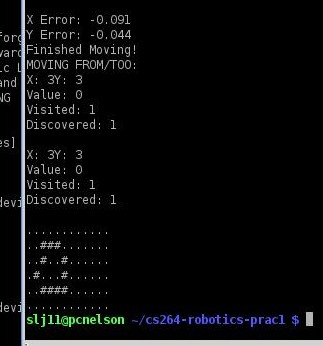
\includegraphics[width=0.5\textwidth]{img/robot_pics/run1_example.jpg}
\caption{Screen shot of the map produced by the trial run shown in the images.}
\label{fig:robot-map-run1}
\end{figure}

\subsection{Hiding the Robot}
Hiding the robot first requires the robot to localize within the map. Unfortunately, because the localization method depends upon the robot being placed in such a way that the robot lines up exactly with the previous grid I could only get the robot to localize with the map if it started in the same square using the previous trial run.

\begin{figure}[H]
\centering
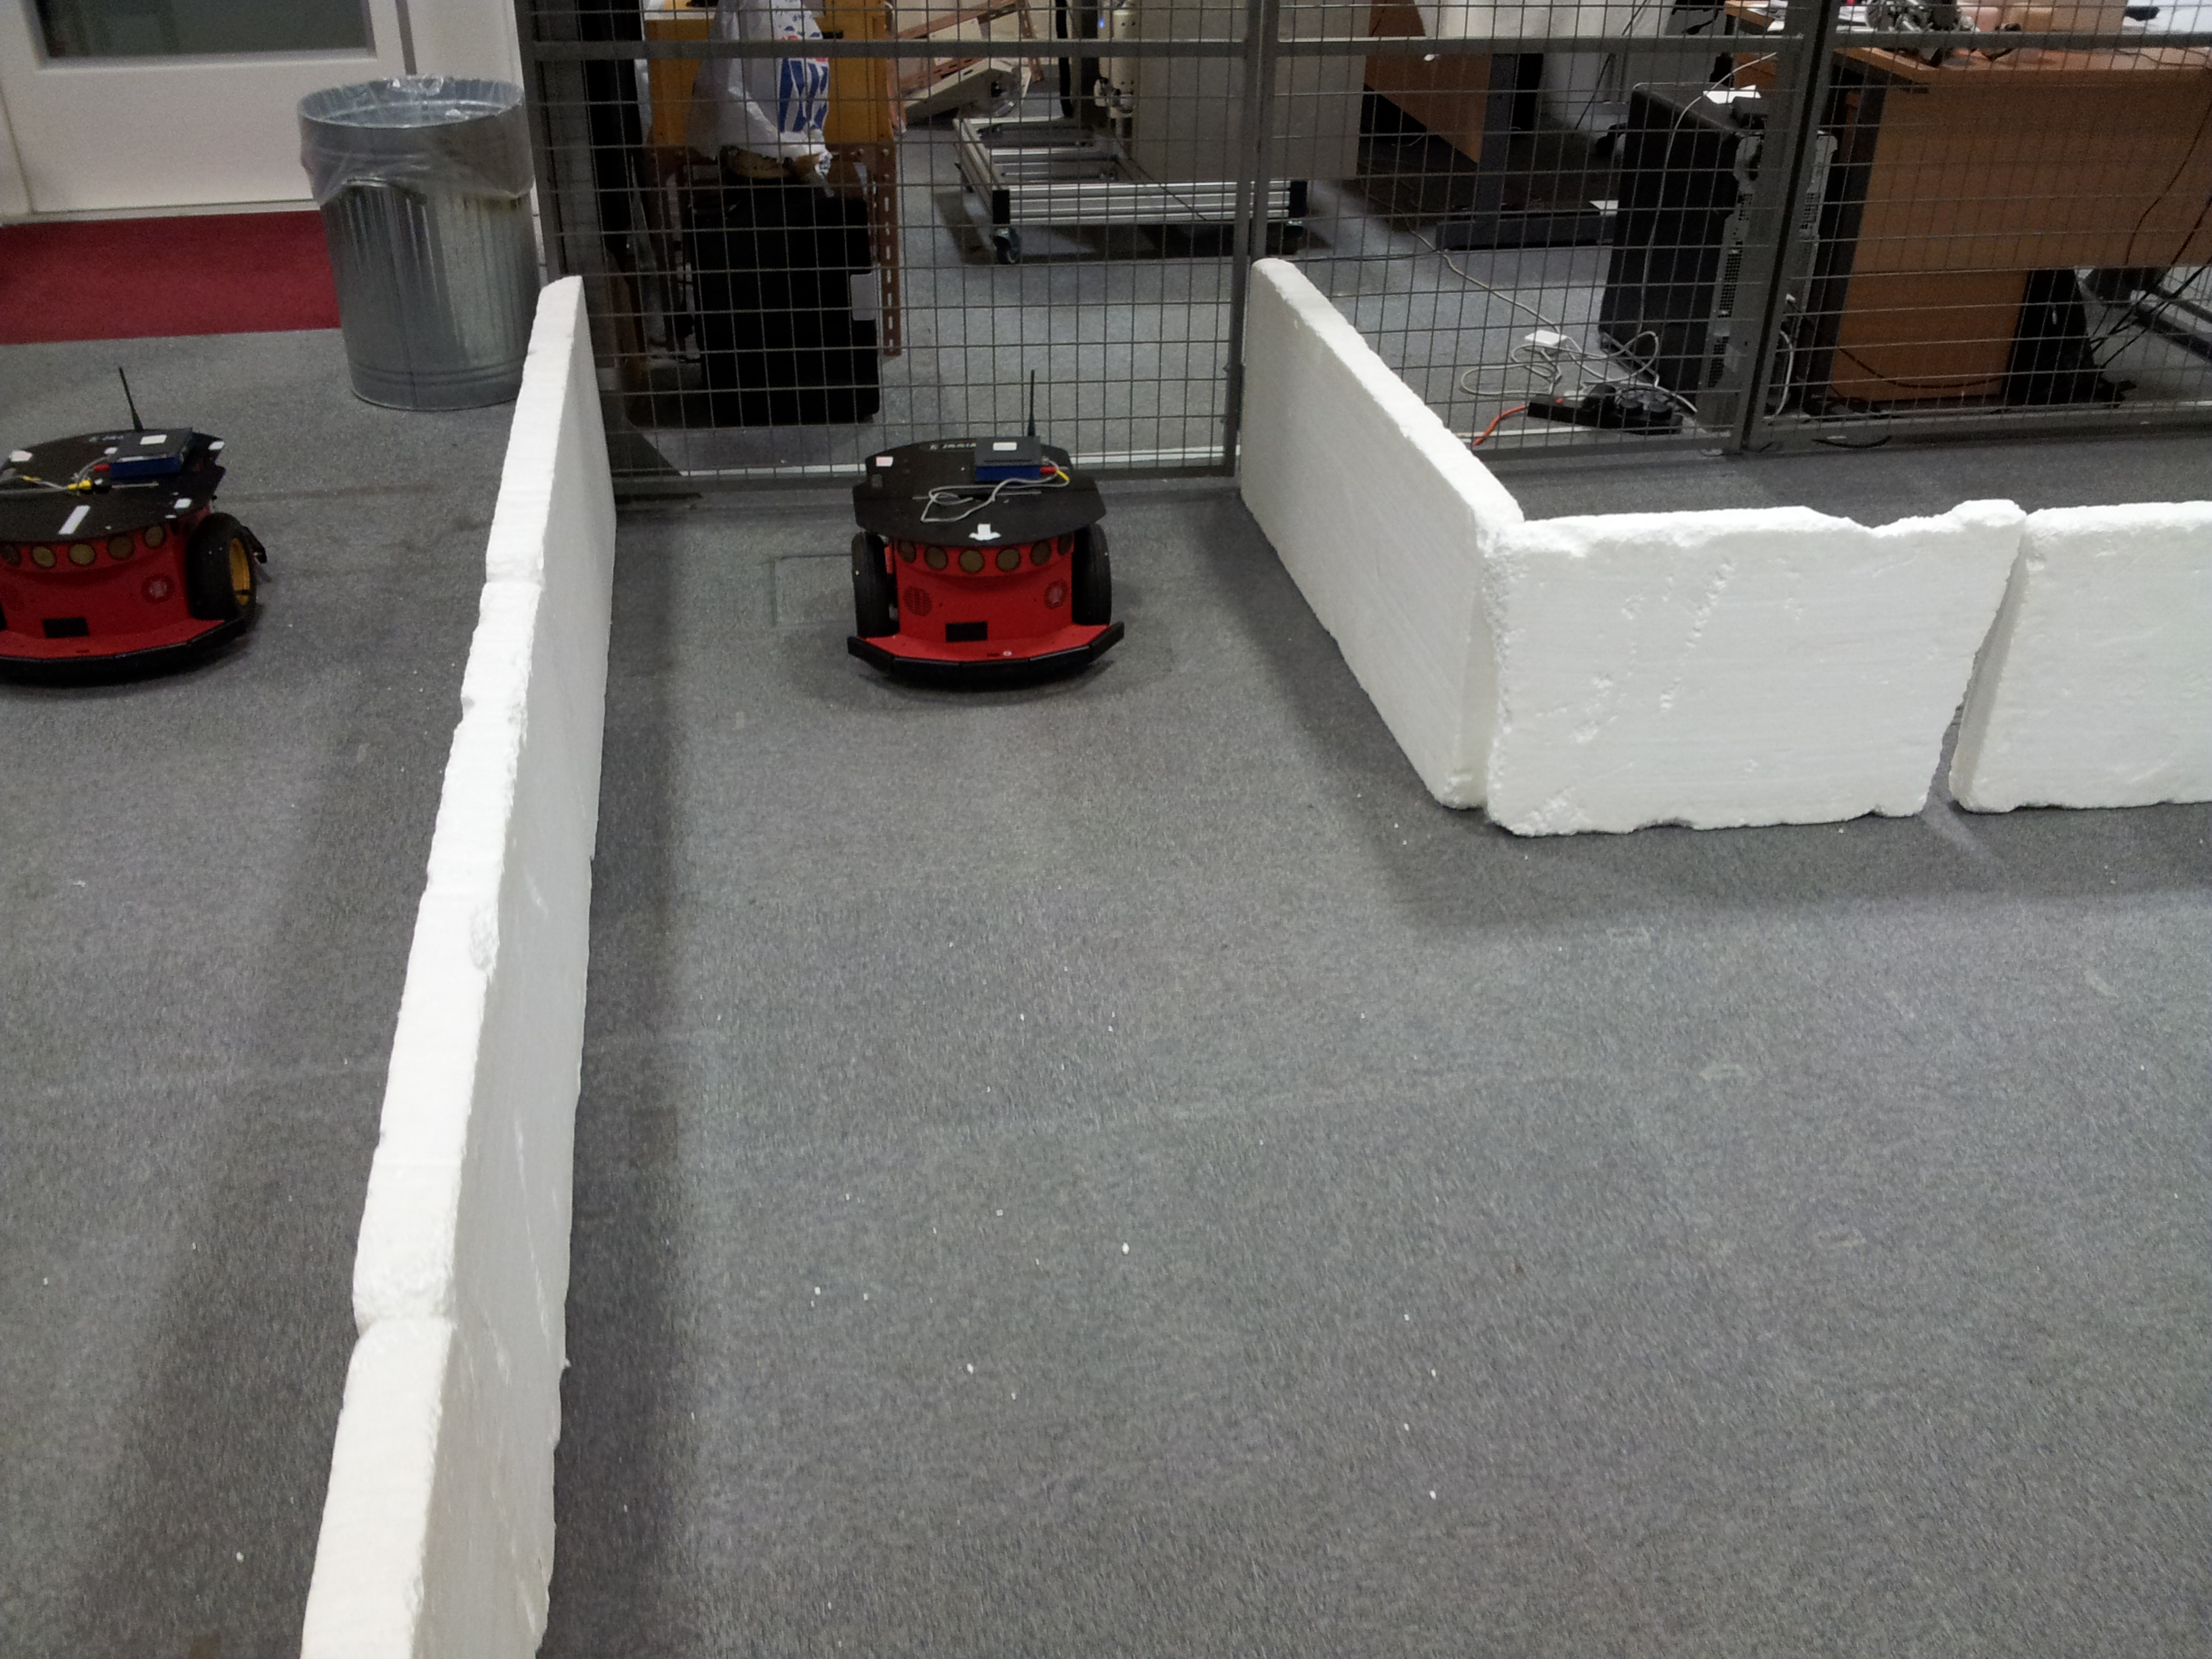
\includegraphics[width=0.4\textwidth]{img/robot_pics/20130416_132228.jpg}
\caption{Pioneer trying to localize at start point in first environment.}
\label{fig:robot-map-localize1-image}
\end{figure}

\begin{figure}[H]
\centering
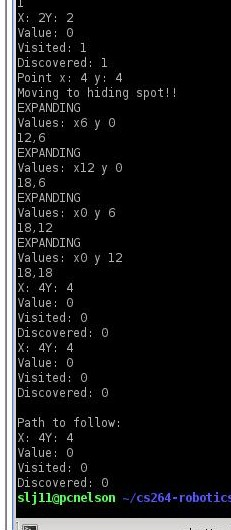
\includegraphics[width=0.4\textwidth]{img/robot_pics/localize1.jpg}
\caption{Screen shot showing a pioneer correctly localizing in a map where the robot starts at the same square (Note that save maps are buffered with 2 cells of padding hence why the robot changes position from (2,2) to (4,4). The hiding spot at the bottom is also (4,4) so the robot does not move.}
\label{fig:robot-map-localize1}
\end{figure}

However when I attempted to localize the robot in a slightly different environment, it did manage to localize the robot in squares outside of the initial start point showing that the concept worked but because of the requirement for the robot to sync up with the pre-defined grid it did not work very well.

\begin{figure}[H]
\centering
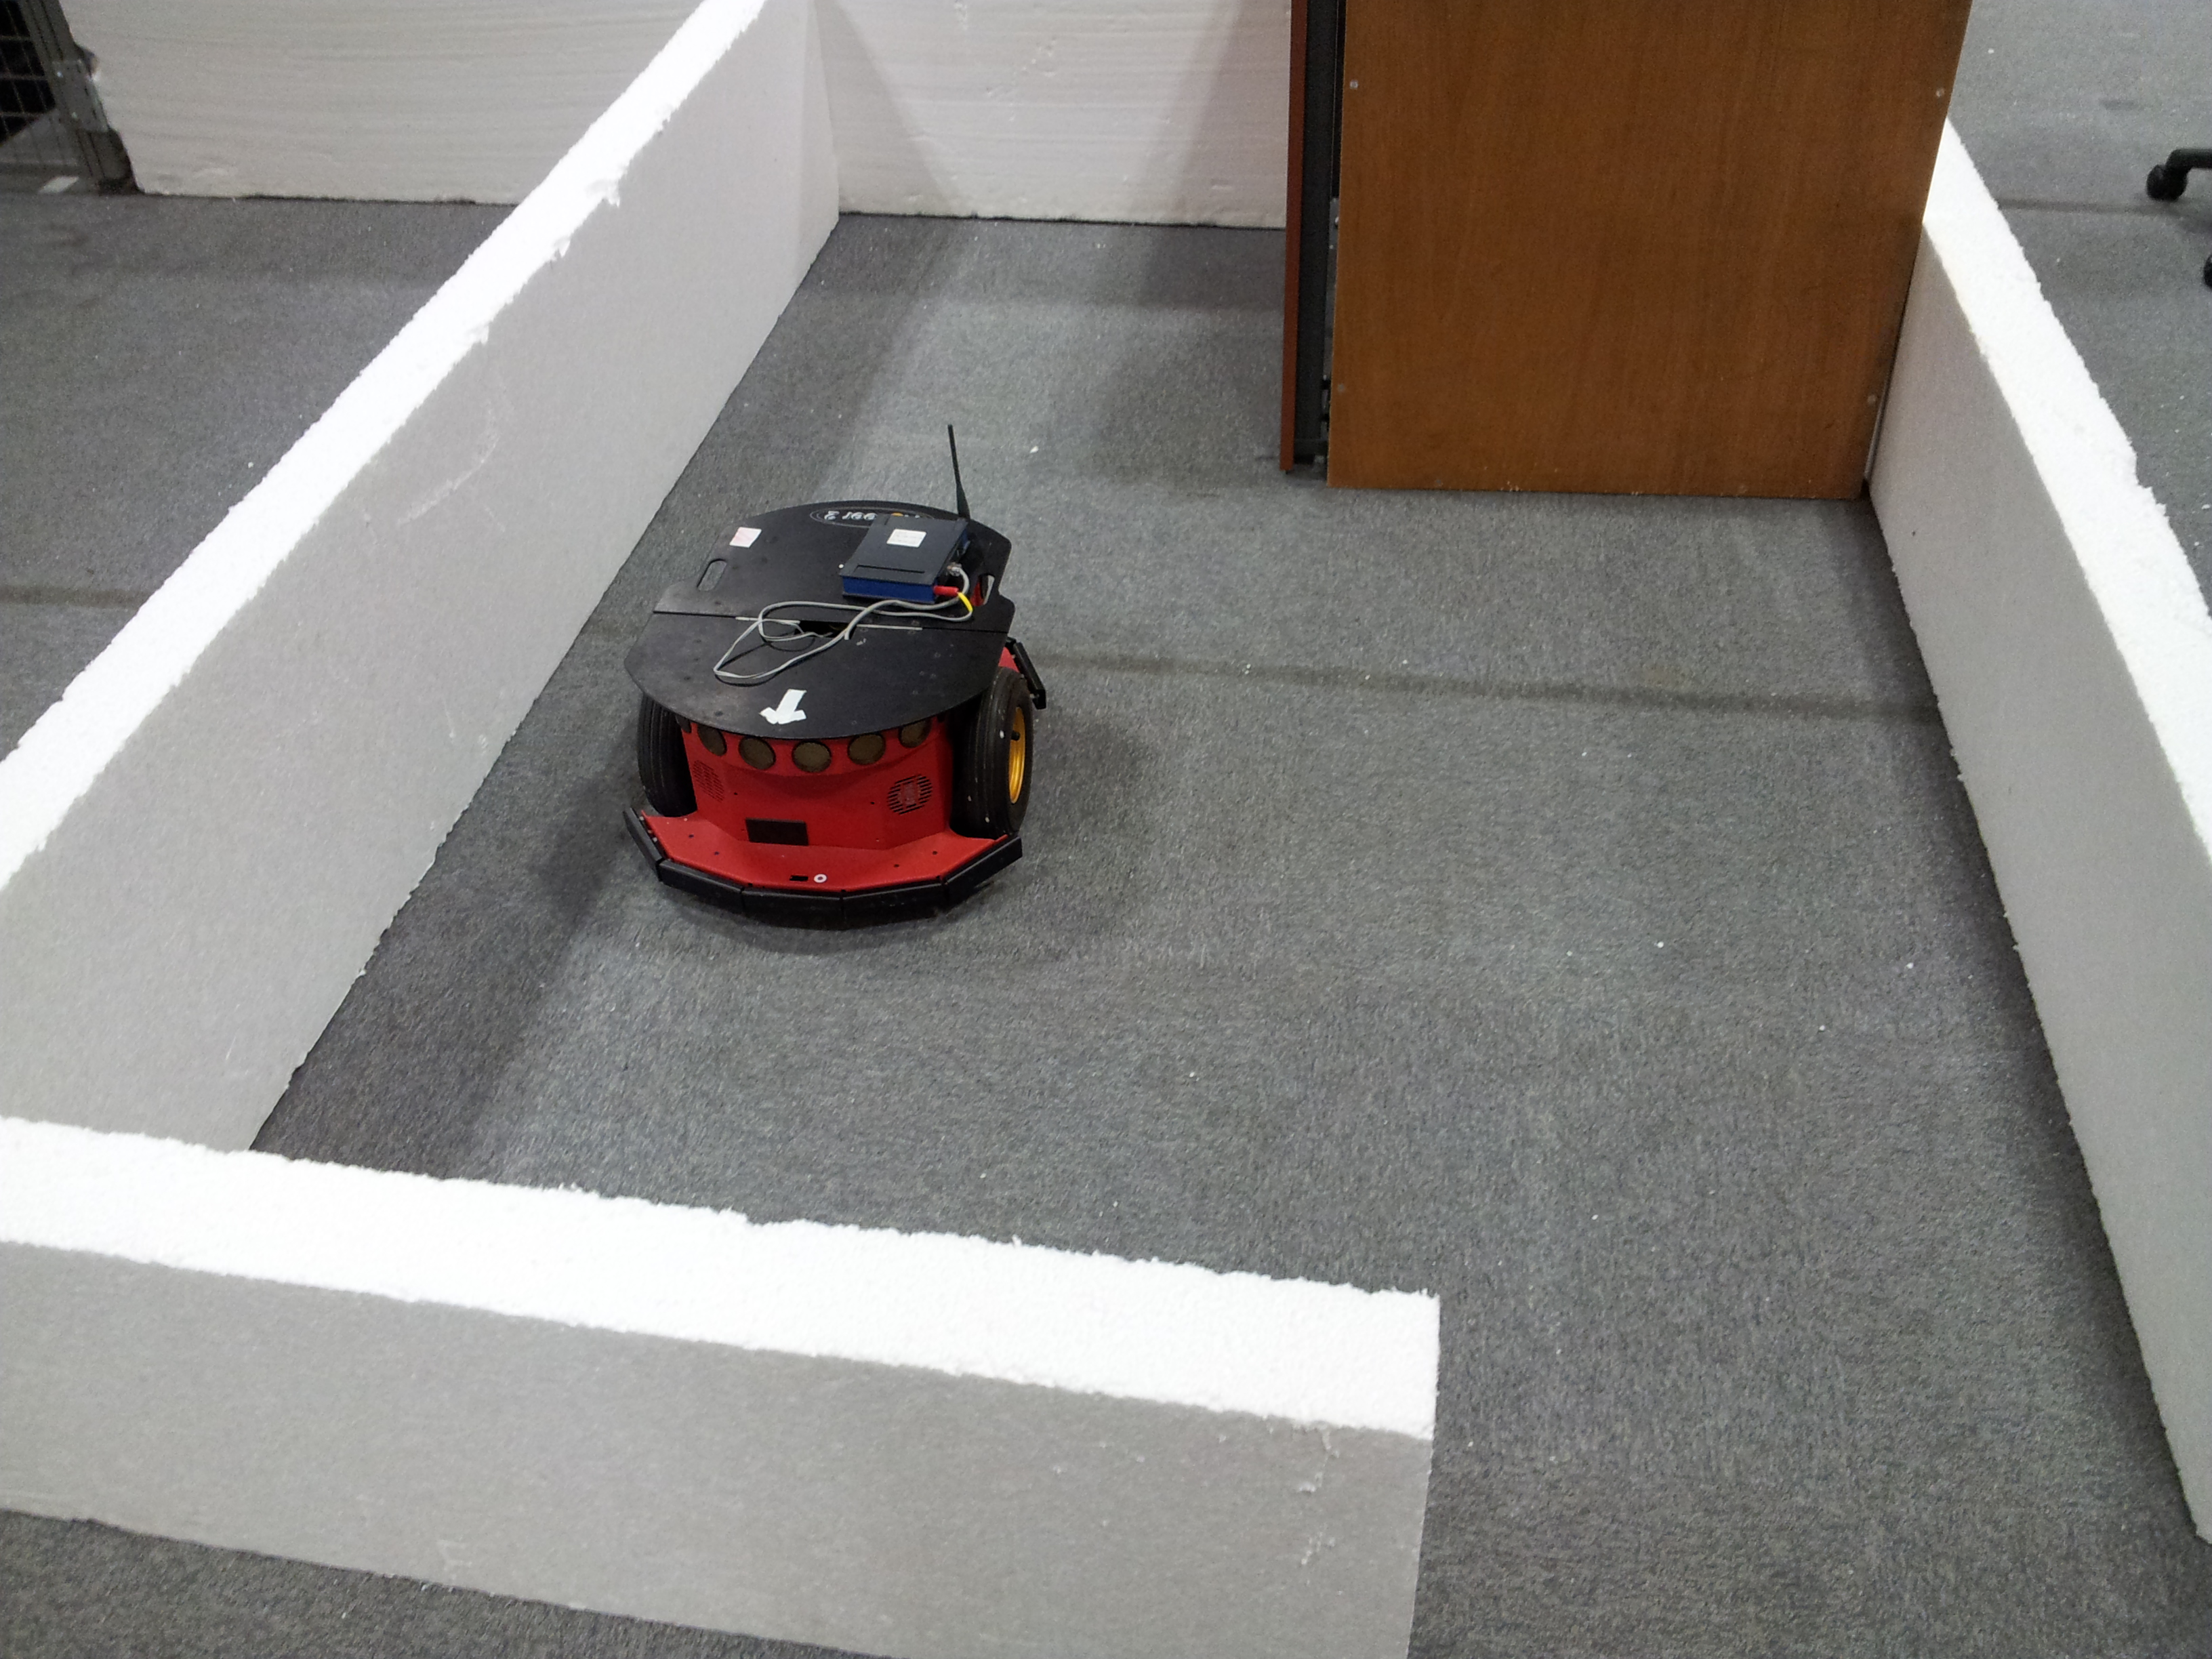
\includegraphics[width=0.5\textwidth]{img/robot_pics/20130416_142622.jpg}
\caption{A Pioneer successfully localizing in another environment. The initial mapping ran from one cell behind (next to the wooden table)}
\label{fig:robot-map-localize2}
\end{figure}

Once the robot had localized, it should of picked a hiding spot from the available squares in the map and then moved to it. The localization attempted in the first example worked even though the robot started in the same place, but it just happened to chose the same cell as it started in as the cell to hide at. This seems logical as in the first trial run the robot started in a corner space. When the robot localized in the second environment it happened to choose a hiding spot outside of the mapped environment. This was due to inaccuracies in the sensor readings and using the wrong threshold. Unfortunately I could not fix this issue in time to attempt another run on the Pioneers.

\subsection{Finding Map Differences}
The final part of the assignment was to identify differences in a map made of the environment. For testing this I used to first environment with an obstacle in place of one of the square. This could represent a hiding robot within the environment.

\begin{figure}[H]
\centering
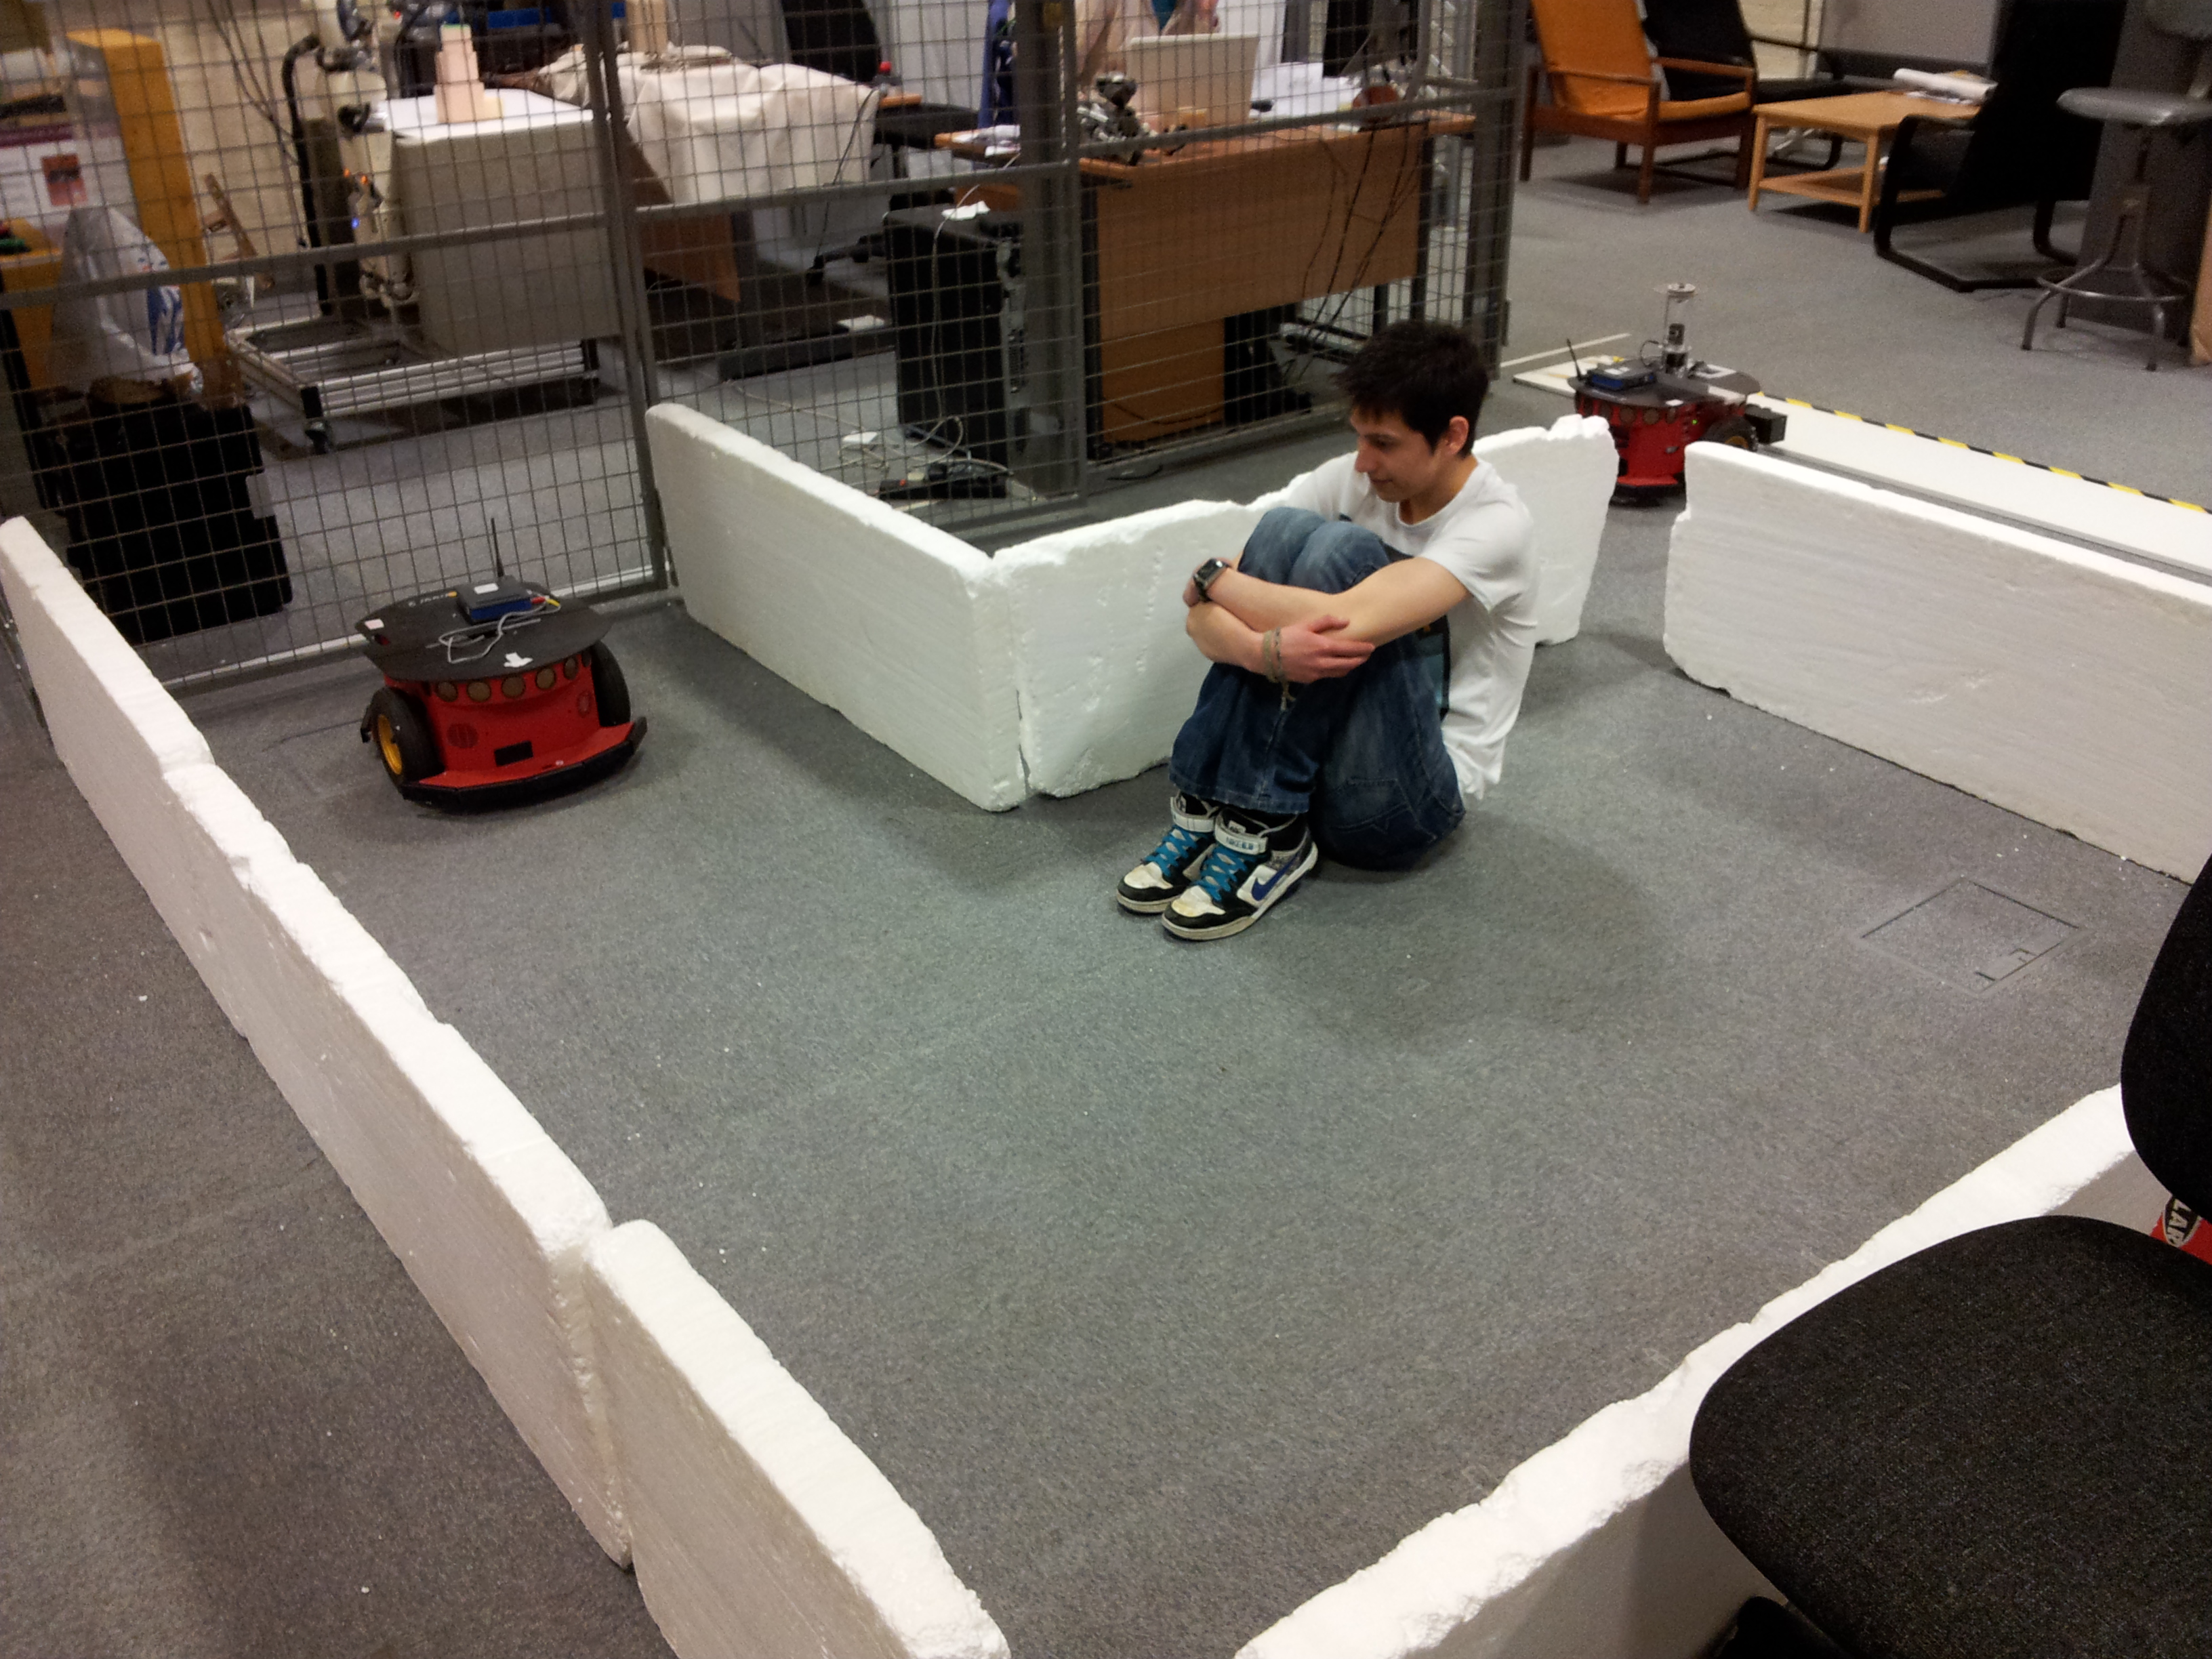
\includegraphics[width=0.5\textwidth]{img/robot_pics/20130416_135014.jpg}
\caption{A Pioneer about to find differences in the map. Complete with obstacle.}
\label{fig:robot-map-obstacle-image}
\end{figure}

\begin{figure}[H]
\centering
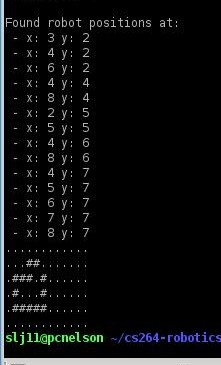
\includegraphics[width=0.4\textwidth]{img/robot_pics/seeker_example.jpg}
\caption{Screen shot after mapping the above environment. Notice the grid differs by one square on the map on the bottom.}
\label{fig:robot-map-obstacle}
\end{figure}

Figure \ref{fig:robot-map-obstacle} shows the output attempting to find points that are different in the map. While you can see that the grid is output with the correct differences at the bottom (compare with screen shot \ref{fig:robot-map-run1}, the number of differences found do not reflect this. I believe this is down to a bug where the map isn't thresholded correctly. Unfortunately I did not have time to fix this bug to get the correct point outputting.

\section{Discussion of Trial Runs}
The trails runs shown in this document could have been a lot better. On the whole I found my robot to be relatively unsuccessful in the real world. However the ideas that underpin the design of the programs is still decent, but is just not smart enough to deal with the complexity of the real world.

For example, the least successful part of the trials was the localization function. This function would work if the robot lined up with the grid in exactly the same way as with the reference map but would fail otherwise. This is because the localization function made no attempt to generalize readings when matching the new grid to the old one. This could be improved by finding a way to compare current and past readings that does not rely on exact matches with the grid, potentially by using probability to measure how closely a new readings match with the reference map.

The mapping of the environment was the part of my application which worked the best. However there were some still a few bugs. Firstly, the map maker program only works when the environment takes the form of Taxicab geometry due to the nature of the occupancy grid and the way the robot moves between cells. Mapping is virtually impossible with diagonally shaped walls or curved walls. Secondly, my cell size was set to use 60x60cm cells which would fit a robot but would be too small to accommodate the robot's turning circle. Making the size of the cells larger would fix this issue but would also decrease the resolution of the map.

Both the hiding and difference detection worked moderately well and had good ideas behind them, however they failed due to some weak coding that wasn't robust enough for the real world. If I'd of had more time to tinker with the robot I believe I could have fixed these errors to give some decent results and got the robot to correctly move to a hiding spot and find a hidden robot in the environment using my existing ideas.

\section{Evaluation of Project}
In conclusion I strongly feel that I approached this assignment from the wrong perspective. If I had to write it again from scratch I would of taken a more reactive approach to the movement and mapping of the robot instead of relying on having to move on a cell by cell basis. The simple random walk that I used in an earlier assignment was able to map the environment far quicker than the approach I used here, but lacked the ability to decided when it had finished mapping. Ideally I would have created a mapper that reactively moved around the environment but had a terminating condition and whose movement was weighted toward unexplored parts of the map. 

I believe that this approach would have allowed me to move around the world quicker and with a great deal less error that with the current approach. While I was happy with the way that the robot moved from point to point and the correction to the movement over time by feeding any error back into the next movement, I feel the movement system could of been better fine tuned using the time integral and better gains to achieve sharper movement, especially when turning.

Additionally, due to the fact that the amount a robot moves is not guaranteed to be perfect and that the internal measure of a position or angle given by the robot software may not even be correct I would of liked to of accounted for this in some way. Possibly by correcting measurements based on the certainty we have about the robots position according to factors such as how far the robot has moved for its initial position.

Localization proved to be the hardest part of the assignment for me. The approach that I took depended far too much on a perfect world. It was also extremely computationally heavy with it having to compare all cells in two grids multiple times. To fix this I would of liked to of incorporated probability regarding potential points that my robot could be at and finding a way to generalize the shape of the new measurements to compare with old measurements. It is worth noting that the approach I took only works if the robot is placed with the same orientation as the reference map. It would of been nice to look into solutions which could handle multiple orientations.

One of the most positive parts of the assignment was the thresholding, which I found to generally work quite well. Otsu's method seemed to reliably separate wall cells and floor cells with decent accuracy. This was useful as it meant that erroneous sensor readings would be removed from the map and corrected for fairly reliably.

As mentioned before I believe that the techniques I have used to find hiding robots and to find and move to hiding spots are both pretty decent, however I believe that the supporting code was not robust enough or not well tested enough and therefore let me down on the real robots. I believe that they could of work fairly well if I had more time to iron out the bugs in this code.

A further point that I would consider changing is how I am using A* to find the shortest path between where I am now and where I wish to hide. At the moment the robot will find the shortest path and blindly follow it to the goal. If I were to write the program again I would still use A* to find the shortest path but perform checks to ensure that the path is still valid and has not changed since the map was created. If something has changed (such as another robot hiding in the environment) I could update the map and perform another A* to find an alternate route round new obstacles.

The biggest lesson learnt from this assignment was that the only perfect model of the world is itself. There are far too many variables in the real world that do not appear in the simulator and therefore cannot be planned for with sufficient testing on real robots. I found that I spent too much time attempting to get highly accurate movement (particularly with turning) when I should have accepted that moderately accurate movement can still be used to achieve the same effect. This would have given me more time to work on other features of the assignment and would of resulted in better trial runs.

In summary, I found this assignment to be one of the most challenging but enjoyable that I have worked on. The design and implementation of robotic controllers is a skill that can only be developed through experience, trial and error, and some clever ideas. I believe that the real world is the only decent measure of controller performance and that simulation can only take the developer so far.

\end{document}